\documentclass[conference]{IEEEtran}
\IEEEoverridecommandlockouts
% The preceding line is only needed to identify funding in the first footnote. If that is unneeded, please comment it out.
\usepackage{cite}
\usepackage{amsmath,amssymb,amsfonts}
\usepackage{algorithmic}
\usepackage{textcomp}
\usepackage{xcolor}
\usepackage{colortbl}
\usepackage[rightcaption]{sidecap}
\usepackage{wrapfig}
\usepackage{adjustbox}
\usepackage{hyperref}
\def\UrlBreaks{\do\/\do-}
\usepackage{graphicx} %package to manage images
\graphicspath{ {./images/} }


\def\BibTeX{{\rm B\kern-.05em{\sc i\kern-.025em b}\kern-.08em
    T\kern-.1667em\lower.7ex\hbox{E}\kern-.125emX}}
\begin{document}

\title{Sistema de Rega Inteligente}

\author{\IEEEauthorblockN{1\textsuperscript{st} Tomás Marcos}
\IEEEauthorblockA{\textit{Faculdade de Ciências Exatas e da Engenharia} \\
\textit{Universidade da Madeira}\\
Funchal, Portugal \\
2037017@student.uma.pt}
\and
\IEEEauthorblockN{2\textsuperscript{nd} Nelson Vieira}
\IEEEauthorblockA{\textit{Faculdade de Ciências Exatas e da Engenharia} \\
\textit{Universidade da Madeira}\\
Funchal, Portugal \\
2080511@student.uma.pt}
}

\maketitle

\begin{abstract}
A água é um recurso precioso, considerado um dos bens essenciais para a vida. 
No entanto, cada vez mais, ouve-se que é um recurso escasso e que rapidamente 
está a se esgotar. A água é utilizada para muitas atividades, sejam elas industriais, 
comerciais ou de lazer. Existem muitas iniciativas que pretendem reduzir o 
consumo e o desperdício de água. Pretendemos explorar um sistema de rega 
inteligente que utilize sensores de forma a reduzir a quantidade de água que 
é utilizada. \\
\end{abstract}

\begin{IEEEkeywords}
IoT, Computação ubíqua, Rega inteligente.
\end{IEEEkeywords}

\section{Introdução}

\IEEEPARstart{A} sustentabilidade global não será alcançada sem garantir a 
disponibilidade de água preciosa para todos os consumidores. Apesar de ser um 
dos principais objetivos da agenda da UN2030 \cite{un2015agenda} para o desenvolvimento 
global sustentável, a atual escassez de água está a crescer rapidamente e 
afetando um número crescente de consumidores de água residencial, comercial, 
industrial e agrícola em todo o mundo \cite{mishra2021water}. Espera-se que a 
procura global da água suba 55\%, enquanto atualmente, cerca de 25\% das grandes 
cidades estão a passar por alguns níveis de stress hídrico \cite{josefine2021differentiated}.

As mudanças climáticas, secas graves, crescimento populacional, aumento da 
procura e má administração durante as últimas décadas enfatizaram ainda mais 
os recursos escassos da água doce em todo o mundo e resultaram numa grave 
escassez de água para cerca de 4 bilhões de pessoas, pelo menos um mês 
anualmente \cite{jafari2018assessing} \cite{unicef2019progress} \cite{orimoloye2021spatial}. \cite{salehi2022global}

Um dos setores de atividade humana que tem maior consumo dos recursos hídricos 
é a agricultura, "aproximadamente 100 vezes mais do que o uso pessoal é consumida 
pela alimentação e agricultura e quase 70\% das águas fluviais e subterrâneas 
são utilizadas na irrigação". \cite{nawandar2019iot} Apenas 17\% das terras 
agrícolas, de todo o mundo são irrigadas. Apesar de por todo o mundo, se verificar 
um aumento de terrenos irrigados, a área irrigada per capita tem estado a diminuir 
desde 1990 devido ao rápido crescimento global. \cite{pimentelwater}

Existem, atualmente, várias tecnologias de irrigação, sendo as mais comuns 
a irrigação por inundação e irrigação por aspersão. Outros métodos mais 
focados, como a irrigação gota-a-gota têm maior eficiência hídrica. Esta 
técnica usa uma quantidade inferior de água, entre 30\% a 50\%, quando 
comparada com uma técnica de irrigação superficial. \cite{pimentelwater}

Várias iniciativas foram tomadas para ajudar a minimizar o desperdício 
de água neste setor, mas, no entanto, não aparentam ter muito sucesso, 
ou não são apelativas, devido aos elevados custos associados. 
Os sensores comerciais para sistemas destinados à agricultura e à sua 
irrigação são muito caros, tornando impossível aos pequenos agricultores 
a implementação deste tipo de sistema nas suas explorações. No entanto, 
os fabricantes oferecem actualmente sensores de baixo custo que podem 
ser ligados a nós para implementar sistemas de baixo custo para a gestão da 
irrigação e monitorização agrícola. Além disso, devido ao interesse em 
sensores de baixo custo para monitorizar a agricultura e a água, 
novos sensores de baixo custo estão a ser propostos em vários estudos. \cite{garcia2020iot}

Portugal Continental, no mês de abril de 2022, encontrava-se numa situação de seca, nos 
quais 81,9\% do território encontrava-se em seca moderada e 17,9\% do território em seca severa, 
segundo o jornal Expresso \cite{expresso}. 

Segundo o Instituto Português do Mar e da Atmosfera (IPMA), 
a quantidade de precitpitação até o dia 15 de abril de 2022, teve um valor médio inferior ao valor normal 
quando comparado com anos anteriores, correspondente a 38\%. Devido à redução da precipitação, 
a percentagem de água no solo diminuiu em quase todo o país com valores inferiores a 20\%, com alguns locais 
a atingirem o ponto de emurchecimento. O boletim também contém um gráfico, demonstrado na figura \ref{fig:ipmagraph} 
que mostra a percentagem de território do país sem situações de seca. \cite{ipmaboletim}

\begin{figure}[h]
    \centering
    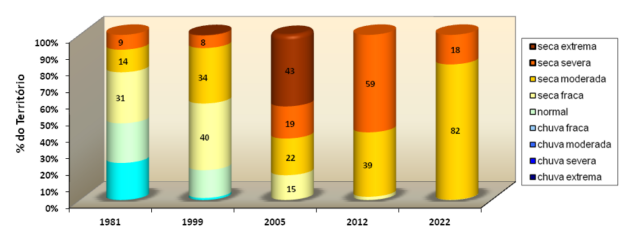
\includegraphics[scale=0.5]{grafico-seca-portugal.png}
    \caption{Percentagem do território de Portugal Continental por classe do índice PDSI em situações de seca anteriores em abril (2022 até dia 15)}
    \label{fig:ipmagraph}
\end{figure}

Por estes motivos é importante gerir o consumo de água no nosso dia a dia, 
portanto o que propomos é um sistema de rega inteligente que faz a 
medição da humidade do solo e rega as plantas apenas durante o tempo 
necessário poupando o gasto desnecessário da água de rega.

\section{Trabalhos Relacionados}

Segundo um estudo realizado por García et al, existem 178 artigos 
relacionados com  "IoT irrigation, IoT irrigation system, and smart 
irrigation" \cite{garcia2020iot}, escritos em inglês, no período de entre os 
anos de 2014 e 2019, inclusive, dos quais 106 artigos estão relacionados com a 
utilização de sensores para monitorizar o estado do solo. Destes 106 artigos 
estudados, todos os artigos abordam a humidade do solo, 9 discutem a temperatura 
do solo, 4 exploram o ph do solo e 3 mencionam os nutrientes presentes no solo.

Na Índia, 10\% da área do país é coberta por plantações de arroz \cite{zampieri2018surface}. 
Além disso, 20\% da população indiana está 
abaixo dos níveis de pobreza e 15\% é insegura em termos alimentares. 
Por conseguinte, a baixa produção alimentar afeta tanto a população como a economia. 
Em 2002, a estação das monções produziu a menor quantidade de precipitação nos 
últimos 130 anos. Isso resultou numa perda da produção de arroz devido à falta 
de água doce. Para determinar a seca causada por anomalias nas águas superficiais, 
foi utilizado o Standardized Precipitation Evapotranspiration Index (SPEI). 
Estes índices e a informação recolhida a partir de sensores que monitorizam o ambiente, 
o solo e a água podem ser utilizados para determinar o estado atual da água e a 
possibilidade de cobrir todas as necessidades de água doce. Os países com maiores 
fundos já implementam sistemas de gestão e reutilização da água com o objetivo de 
otimizar a utilização da água e reduzir o impacto ambiental causado pela utilização 
de grandes quantidades de água. No entanto, alguns países podem considerar que estas 
soluções são dispendiosas. 
Os sensores comerciais para sistemas destinados à agricultura e à sua irrigação 
são muito caros, impossibilitando aos pequenos agricultores a implementação deste 
tipo de sistema nas suas explorações. No entanto, os fabricantes oferecem atualmente 
sensores de baixo custo que podem ser ligados a nós para implementar sistemas de baixo 
custo para a gestão da irrigação e monitorização agrícola. Além disso, devido ao interesse 
em sensores de baixo custo para monitorizar a agricultura e a água, estão a ser propostos 
novos sensores de baixo custo em investigações tais como um sensor de monitorização do 
stress hídrico foliar \cite{daskalakis2018}, um sensor de humidade do solo de vários níveis composto 
por anéis de cobre colocados ao longo de um tubo de PVC \cite{guruprasadh2017intelligent}, 
um sensor de monitorização da salinidade da água feito com bobinas de 
cobre \cite{parra2013low} ou um sensor de turbidez da água 
feito com emissores e recetores de chumbo colorido e infravermelho \cite{sendra2013low}.

Devido aos recentes avanços nos sensores para a implementação de sistemas de 
irrigação para a agricultura e à evolução das tecnologias WSN e IoT que podem ser 
aplicadas no desenvolvimento destes sistemas, apresentamos um estudo destinado a resumir 
o estado atual da arte em matéria de sistemas de irrigação inteligentes. Neste inquérito, 
vamos fornecer uma visão geral do estado da investigação relativa aos sistemas de irrigação. 
Iremos determinar os parâmetros que são monitorizados nos sistemas de irrigação 
relativamente à quantidade e qualidade da água, características do solo, condições 
meteorológicas e utilização de fertilizantes. Forneceremos uma visão geral dos nós mais 
utilizados e das tecnologias sem fios empregados para implementar sistemas de irrigação 
inteligentes baseados em WSN e IoT. Finalmente, discutiremos os desafios e as melhores 
práticas para a implementação de sistemas de irrigação baseados em sensores.





Nas actividades agrícolas que utilizam insumos de água, também conhecidas como 
agricultura irrigada, existem diferentes maneiras de distribuir a água. 
As diferentes opções apresentam eficiência diferente e, em alguns casos, 
uma forma específica deve ser utilizada para uma cultura específica. 
As formas específicas de irrigação têm uma grande variedade, mas podemos 
dividi-las nas seguintes categorias: Podemos considerar a forma de distribuição da água: 
(i) irrigação por inundação, (ii) irrigação por aspersão, (iii) irrigação por gotejamento, 
e (iv) irrigação por nebulização. Quanto à existência de sistemas de detecção, podemos ter: 
(i) irrigação sem qualquer consideração, quando a quantidade de água não é calculada ou estimada, 
(ii) irrigação programada, quando a água é fornecida de acordo com as necessidades 
estimadas num período do ano, (iii) irrigação ad hoc, quando a quantidade de água 
é calculada com base nas medições dos sensores. A grande maioria dos artigos incluídos 
nesta secção propõe a utilização de bombas e válvulas para distribuir a água em conjunto 
com sensores para medir os parâmetros ambientais, a fim de calcular as necessidades de água. 
Dos 89 artigos avaliados nesta secção, 83 incluem informações claras sobre o sistema de 
irrigação proposto, os outros seis apenas mencionam que incluem actuadores para irrigação, 
ver Figura 3. Estes 83 incluem diferentes níveis de detalhe, existem 49 documentos que apenas 
indicam que existem motores/bombas no seu sistema (40 documentos) ou válvulas 
(nove documentos) sem mais detalhes. Dos documentos que oferecem mais pormenores, 
19 incluem aspersores (o sistema mais utilizado) \cite{gonzalez2018iot, ahmed2016intelligation, yusuf2005information, cambra2017iot, arvind2017automated, ammour2018factory, singh2019iot, wu2016secure, solanki2017conceptual, wasson2017integration, johar2018iot, ryu2015design, reche2014smart, chieochan2017internet, arumugam2018internet, boonchieng2018smart, rawal2017iot, guo2015design, khattab2016design}, 
oito utilizam irrigação por gotejamento \cite{daskalakis2018uw, nawandar2019iot, barkunan2019smart, sivaprasath2016arduino, kumar2017internet, kodali2016iot, abidin2015web, banumathi2017android}, dois propõem a 
utilização de pulverizadores \cite{mechsy2017mobile}, e os restantes utilizam um sistema de irrigação 
muito específico (robts \cite{rahul2018iot}, pivot, pistola de chuva \cite{vasu2017intelligent} 
ou pode ser aplicada a múltiplos sistemas \cite{agale2017automated}). Em conjunto com o sistema de irrigação principal, 
três papéis propõem o uso de um sistema de nebulização [41,43,51] e dois papéis 
propõem o uso de fertirrigação nos seus sistemas [42,52]. 

Dos artigos que mencionam o tipo de sensor utilizado, o sensor mais popular é o 
e YL69 (SparkFun Electronics, Niwot, CO, USA). Este sensor tem um baixo custo e 
foi criado para operar especificamente com o Arduino. \cite{garcia2020iot}

Muitos sistemas de rega inteligente têm por base sensores de humidade so solo, como 
é o caso dos sistemas que vamos analisar de seguida.

\subsection{Caso de Abbas}

No estudo realizado por Abbas et al. \cite{abbas2014smart}, os autores propõem 
um sistema de irrigação inteligente no qual utilizaram uma rede de sensores sem 
fios para detetar a humidade no solo. Um dos focos do estudo proposto foi a medição 
do tempo de resposta e a capacidade do sistema identificar a capacidade de 
retenção de água do tipo de solo no qual os sensores estavam localizados. 
No entanto, os autores referem que seria necessário ter em consideração outros 
aspetos, tais como a estação do ano, pois no Verão, é necessário regar as plantas 
com maior freqência.

\subsection{Caso de Goap}

Muitos sistemas de rega inteligente têm por base sensores de humidade so solo, como 
é o caso do sistema proposto por Goap et al \cite{goap2018an} em que 

A humidade do solo é um parâmetro crítico para o desenvolvimento para inteligente
Sistema de Rigação. A umidade do solo é afetada por vários ambiente
variáveis mentais, por exemplo, temperatura do ar, umidade do ar, UV, solo
Peratura, etc. com avanço nas tecnologias, o clima
A precisão da previsão melhorou significativa e o clima para sempre
Os dados fundidos podem ser usados para previsão de alterações na umidade do solo.
Este artigo é uma arquitetura de irrigação inteligente baseada em IoT junto
com uma abordagem baseada em aprendizado de máquina híbrida para prever o solo
Umidade. O algoritmo proposto usa os dados dos sensores do passado recente e
A data prevista para a previsão da umidade do solo da próxima
Dias. O valor previsto da umidade do solo é melhor em termos de seus
Precisão e taxa de erro. Além disso, a abordagem de previsão é integrada
Protótipo do sistema independente. O protótipo do sistema é custa ef-
FECTIVO, It é baseado nas tecnologias padrão abertas. O modo automático
O torna um sistema inteligente e pode ser ainda mais personalizado para aplicação
Cenário específico.

\section{Métodos e Metadologias}

O trabalho descrito neste artigo pertende responder a algumas questões que foram 
levantadas após alguma investigação sobre soluções já existentes no que diz respeito 
a sistemas de rega. O sistema proposto permite poupar água? Qual a quantidade de água 
que é possível poupar?  Qual é o custo associado à integração de sensores num sistema 
de rega convencional? Em comparação com um sistema de rega convencional, 
qual a poupança que um sistema de rega inteligente proporciona?

\subsection{O nosso sistema}

O sistema de rega inteligente que propomos faz uso do Arduino MKR 1000 WiFi, 
de um sensor de humidade do solo, modelo 123, de uma breadboard, de vários LEDs 
e uma resistência de 200 ohms. Decidimos usar este modelo do Arduino pela ligação 
à rede por Wi-fi que possui, o que nos permite analisar o sistema sem termos de 
estar no local da instalação, o que podemos fazer através do Arduino Cloud, 
que envia-nos os resultados do sensor que estamos a usar. Caso o utilizador 
queira ver o estado da humidade do solo, pode perceber pelos LEDs que usamos no sistema, 
estes LEDs mostram um feedback visual do estado atual do solo, decidimos representar este 
feedback com 5 LEDs de várias cores que vão desde o verde até ao vermelho, portanto 
se o LED verde estiver acesso quer dizer que o solo está suficientemente humido, se 
o LED laranja estiver acesso quer dizer que solo requer um pouco de água e se o LED
vermelho estiver acesso quer dizer que o solo está seco, e por isso tem que ser regado.

O dispositivo Arduino, como mostra a figura \ref{fig:circuit}, que usamos é o 
modelo MKR 1000 WiFi pois é um modelo com capacidade wifi, o que facilita na 
transmissão dos dados para o utilizador que poderá vê-los no seu smartphone, 
esta interação com o smartphone não foi criada mas é uma possibilidade, bem 
como a utilização de um Raspberry Pi para fazer o tratamento da informação 
recebida pelo Arduino.

O sensor de humidade, ilustrado pela figura \ref{fig:circuit}, é um 
sensor normal para esta função, que tem por base valores entre 0 e 1023, serão usados valores 
incrementais entre os valores mínimo e máximo para fazer uma distinção do grau 
de escassez do solo, a partir destes valores base associamos uma percentagem 
que irá corresponder à humidade do solo, a utilização de percentagem é 
mais user-friendly e consequentemente o sistema dará um feedback mais útil
para o utilizador. Também poderia ser usado um Raspberry Pi para guardar dados do sensor.

Testou-se o sistema com dois sensores de humidade, mas não se observou variações de valores significativas, 
sendo que a distinção dos sensores considerou-se não ser relevante.

\begin{figure}
    \centering
    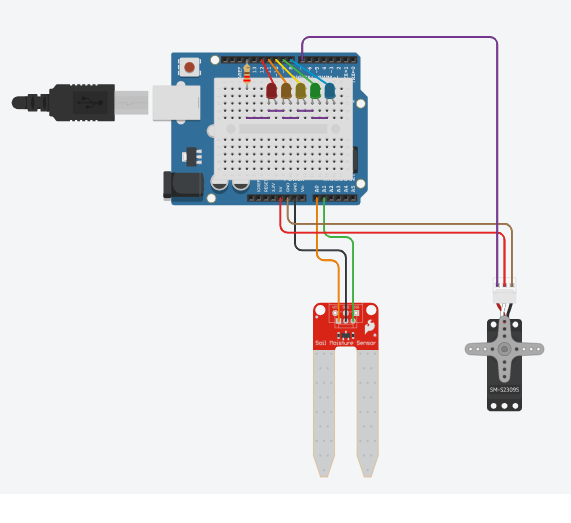
\includegraphics[scale=0.5]{soil-moisture-circuit-schema.png}
    \caption{Esquema do Circuito}
    \label{fig:circuit}
\end{figure}

\subsubsection{Preço do sistema}

Na Tabela \ref{pricetable} podemos verificar o custo do sistema, 
isto inclui apenas os custos associados aos sensores e equipamento 
estritamente necessário à criação deste sistema, portanto custo associados 
a produtos ou serviços externos não são considerados para esta análise, 
como por exemplo o custo de água gasta, pois estes valores variam ao longo 
do tempo e por região e seria difícil fazer uma estimativa para tal.

\begin{table}[ht]
\centering
\small
\begin{tabular}{|c|c|c|c|c|}
    \hline
    \rowcolor{gray}
    \color{white}Item & \color{white}Preço \\
    \hline
    Arduino MKR 1000 WiFi & 30,70 € \\
    \hline
    Sensor de humidade & 5,40 € \\
    \hline
    Servo motor & 5,10 € \\
    \hline
    LEDs & 13 € (Pack) \\
    \hline
    Resistência & 6 € (Pack de 100) \\
    \hline
    Fios e outros cabos e Breadboard & 7,00 \\
    \hline
    \rowcolor{gray}
    \color{white}Total & \color{white}67,20 € \\
    \hline
\end{tabular}
\vspace{1em}
\caption{Custo do material utilizado}
\label{pricetable}
\end{table}

Como podemos verificar o custo total deste sistema, ou de um sistema de 
rega inteligente similar, não é muito elevado. Apesar de ser difícil estimar 
um valor concreto para o custo de água gasta podemos assumir que seria um custo 
muito mais baixo do que é no momento para um utilizador que não use um sistema de 
rega inteligente, pois este tipo de sistema está desenhado para poupar água. 
Comparando com alguns sistemas de rega inteligente que existem no 
mercado \cite{amazonOrbit} \cite{amazonNetro}, o nosso sistema é mais barato e 
atendendo ao facto de que os preços descritos na tabela \ref{pricetable} incluem packs de 
produtos e a utilização do servo motor neste sistema é para efeitos de simulação 
de uma bomba de água, o preço real do sistema seria ainda mais barato, o preço mais 
baixo poderia ser por volta de 40 €, o que tornaria este sistema atraente para 
potenciais consumidores interessados na sustentabilidade e na redução da sua pegada 
ambiental.

\subsection{Testes ao sistema}

Realizamos vários testes, tanto num ambiente controlado como em ambiente real, desde 
a construção do circuito em simulação até ao momento de entrega final. Começamos 
por fazer testes simulados, para isso usamos a ferramenta Tinkercad \cite{tinkercad} onde 
criamos o circuito e o código associado ao circuito que implementa a lógica 
que o sistema deve seguir, neste ambiente de simulação é possível testar 
o sistema de forma a verificar se o código criado faz realmente aquilo 
que é pretendido.

Num dos testes do primeiro protótipo do sistema, no qual apenas se tinha o microcontrolador
Arduino Uno e o sensor de humidade, foi possível observar que o valor máximo obtido pelo sensor 
era de 1023, quando o recipiente com terra continha demasiada água. Este teste, por ainda 
não se ter implmentado todo o circuito considerou-se ser um teste preliminar.

\begin{figure}[h]
    \centering
    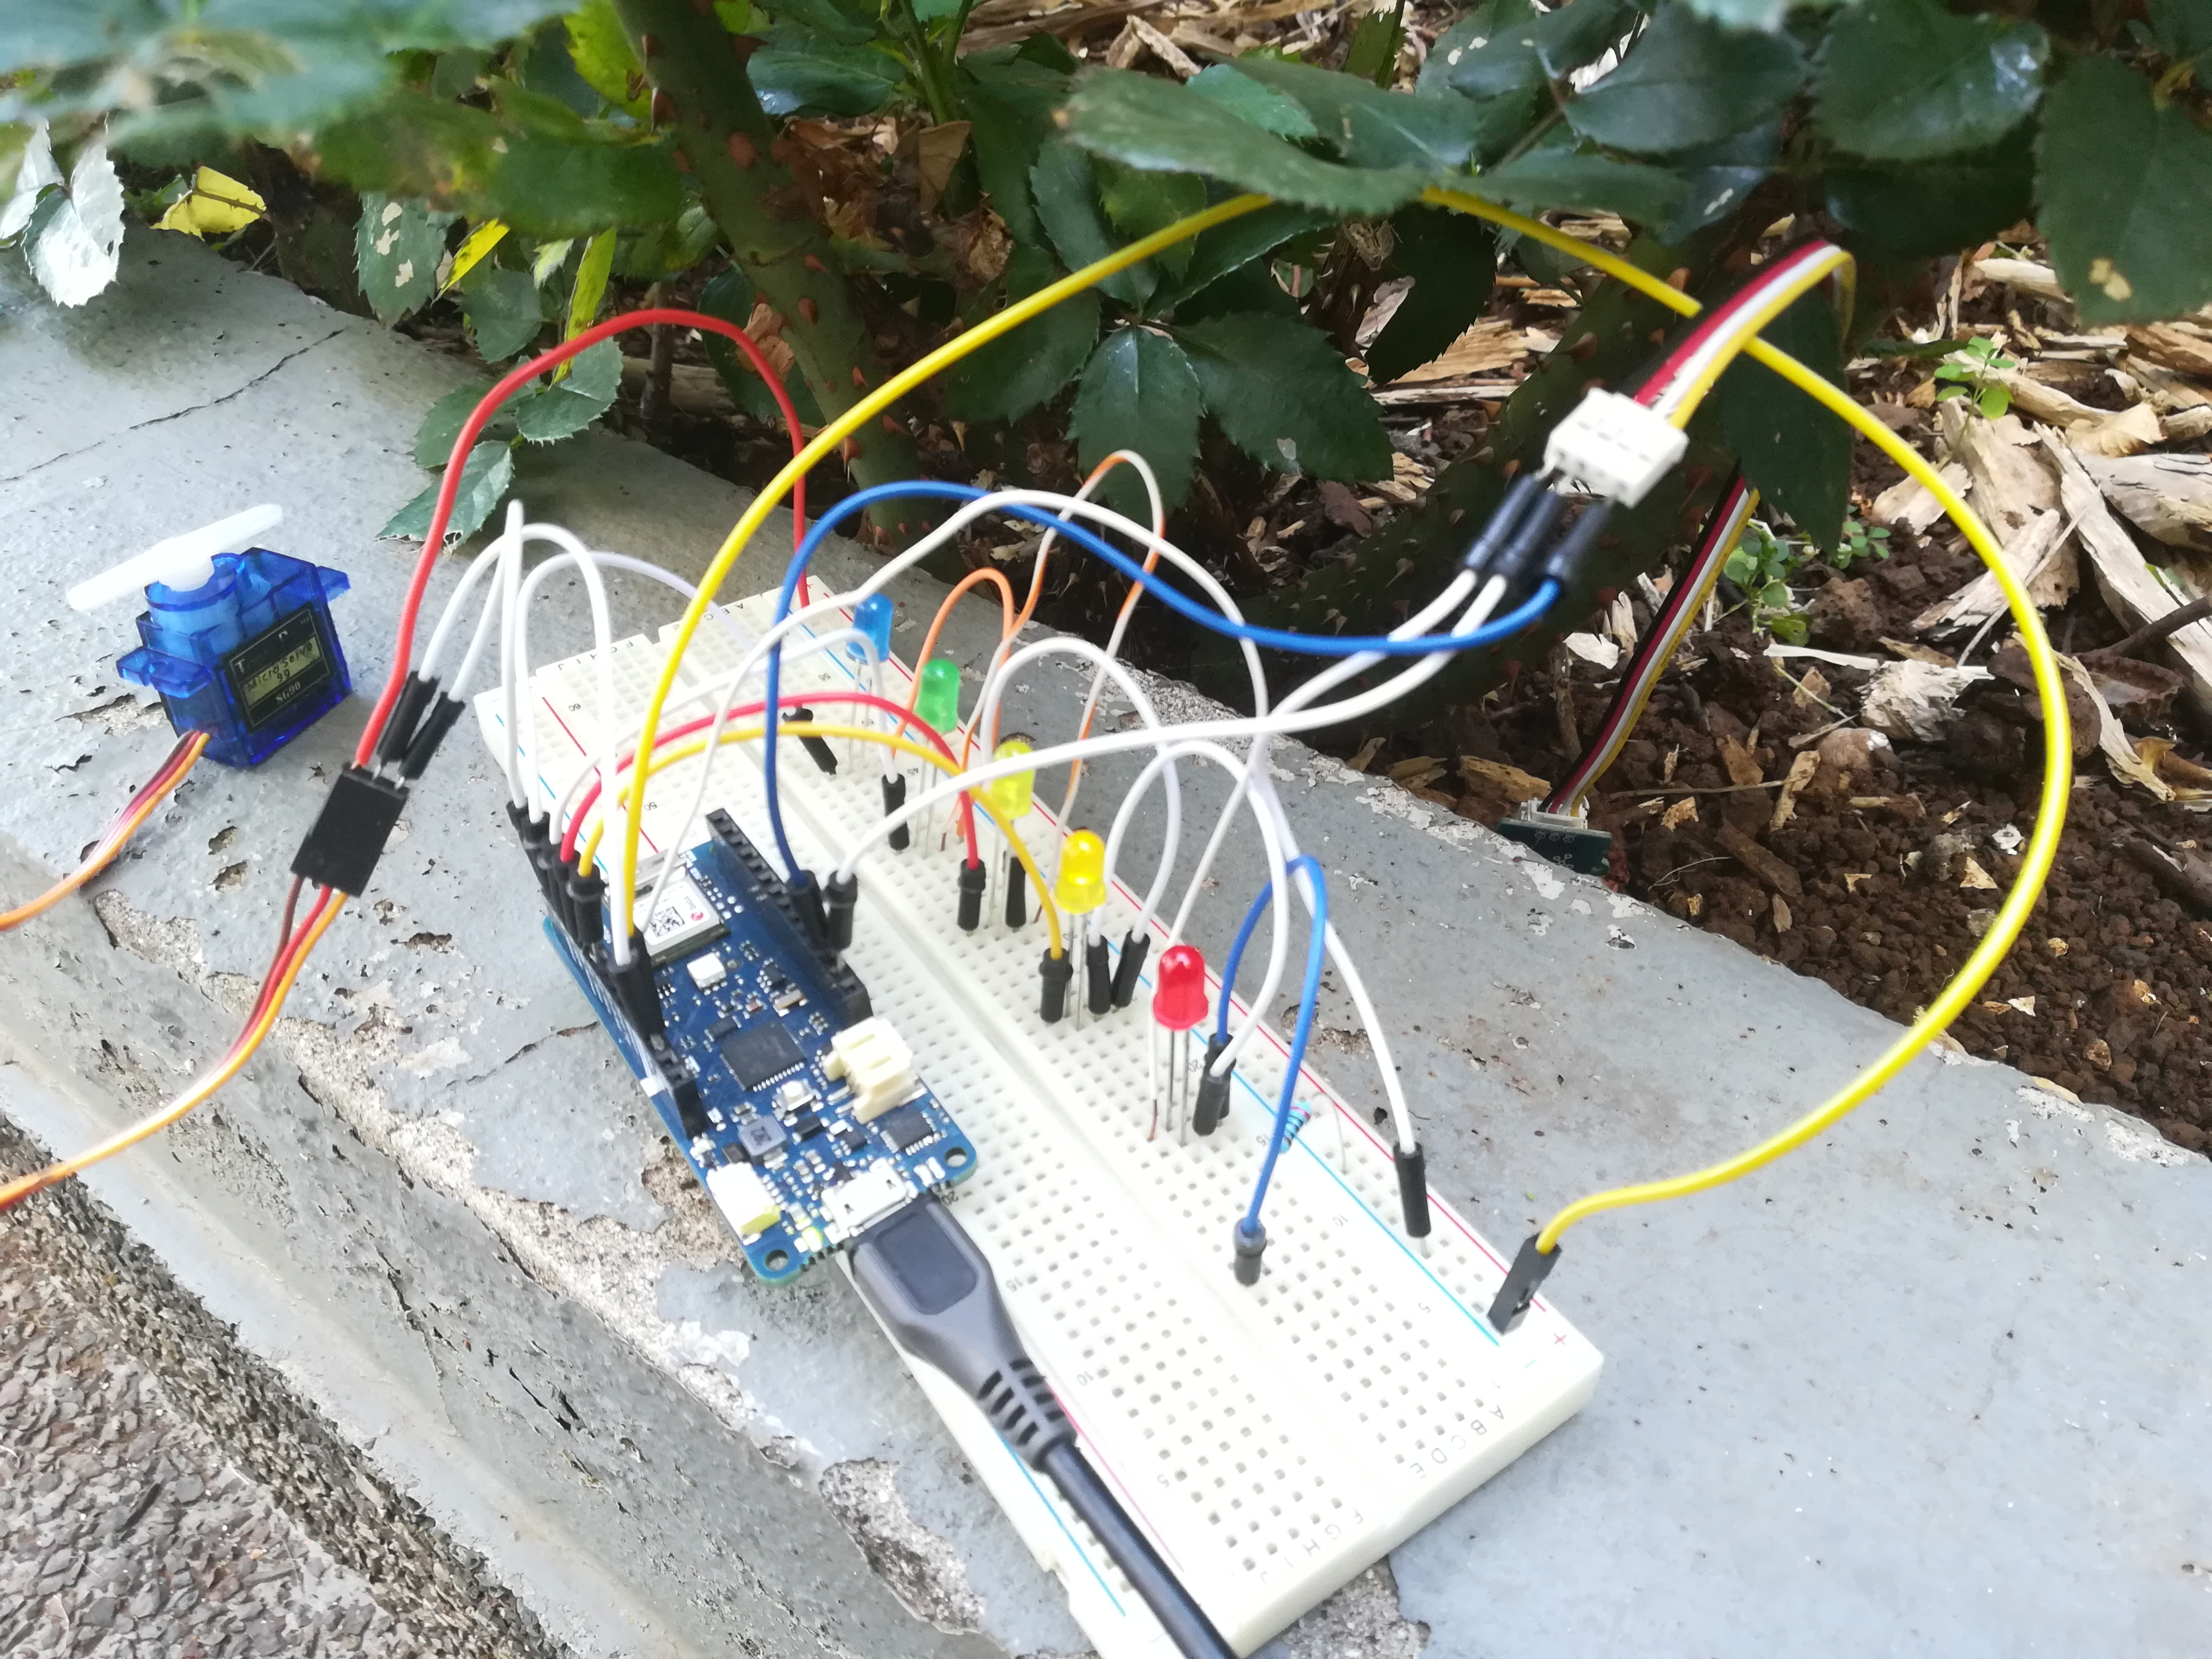
\includegraphics[scale=0.06]{sistema-de-rega-teste-ambiente-real.jpg}
    \caption{Teste realizado}
    \label{fig:teste}
\end{figure}

Posteriormente, realizou-se vários testes no jardim de um dos discentes, como mostra a figura \ref{fig:teste}, 
no qual os resultados obtidos num dos testes, podem ser verificados pelo gráfico da figura \ref{fig:graphic}. 

Como se pode observar pelo gráfico, os valores iniciais estão comprimidos entre os 280 e os 300, 
havendo uma descida abruta logo após se ter iniciado o teste. Isto deve-se ao facto de se ter começado 
o processo de irrigação. O solo por estar seco começou a absorver água e o sensor perdeu alguma estabilidade.
Após, cerca de 1 minuto, verificou-se uma subida constante no valor da humidade do solo até se atingir 
um valor máximo de 400. Após se atingir este pico, os valores estabilizaram-se, havendo uma pequena variação 
nos valores da humidade. Deixou-se de regar a planta e observou-se que os valores da humidade, começaram 
a diminuir.

\begin{figure}
    \centering
    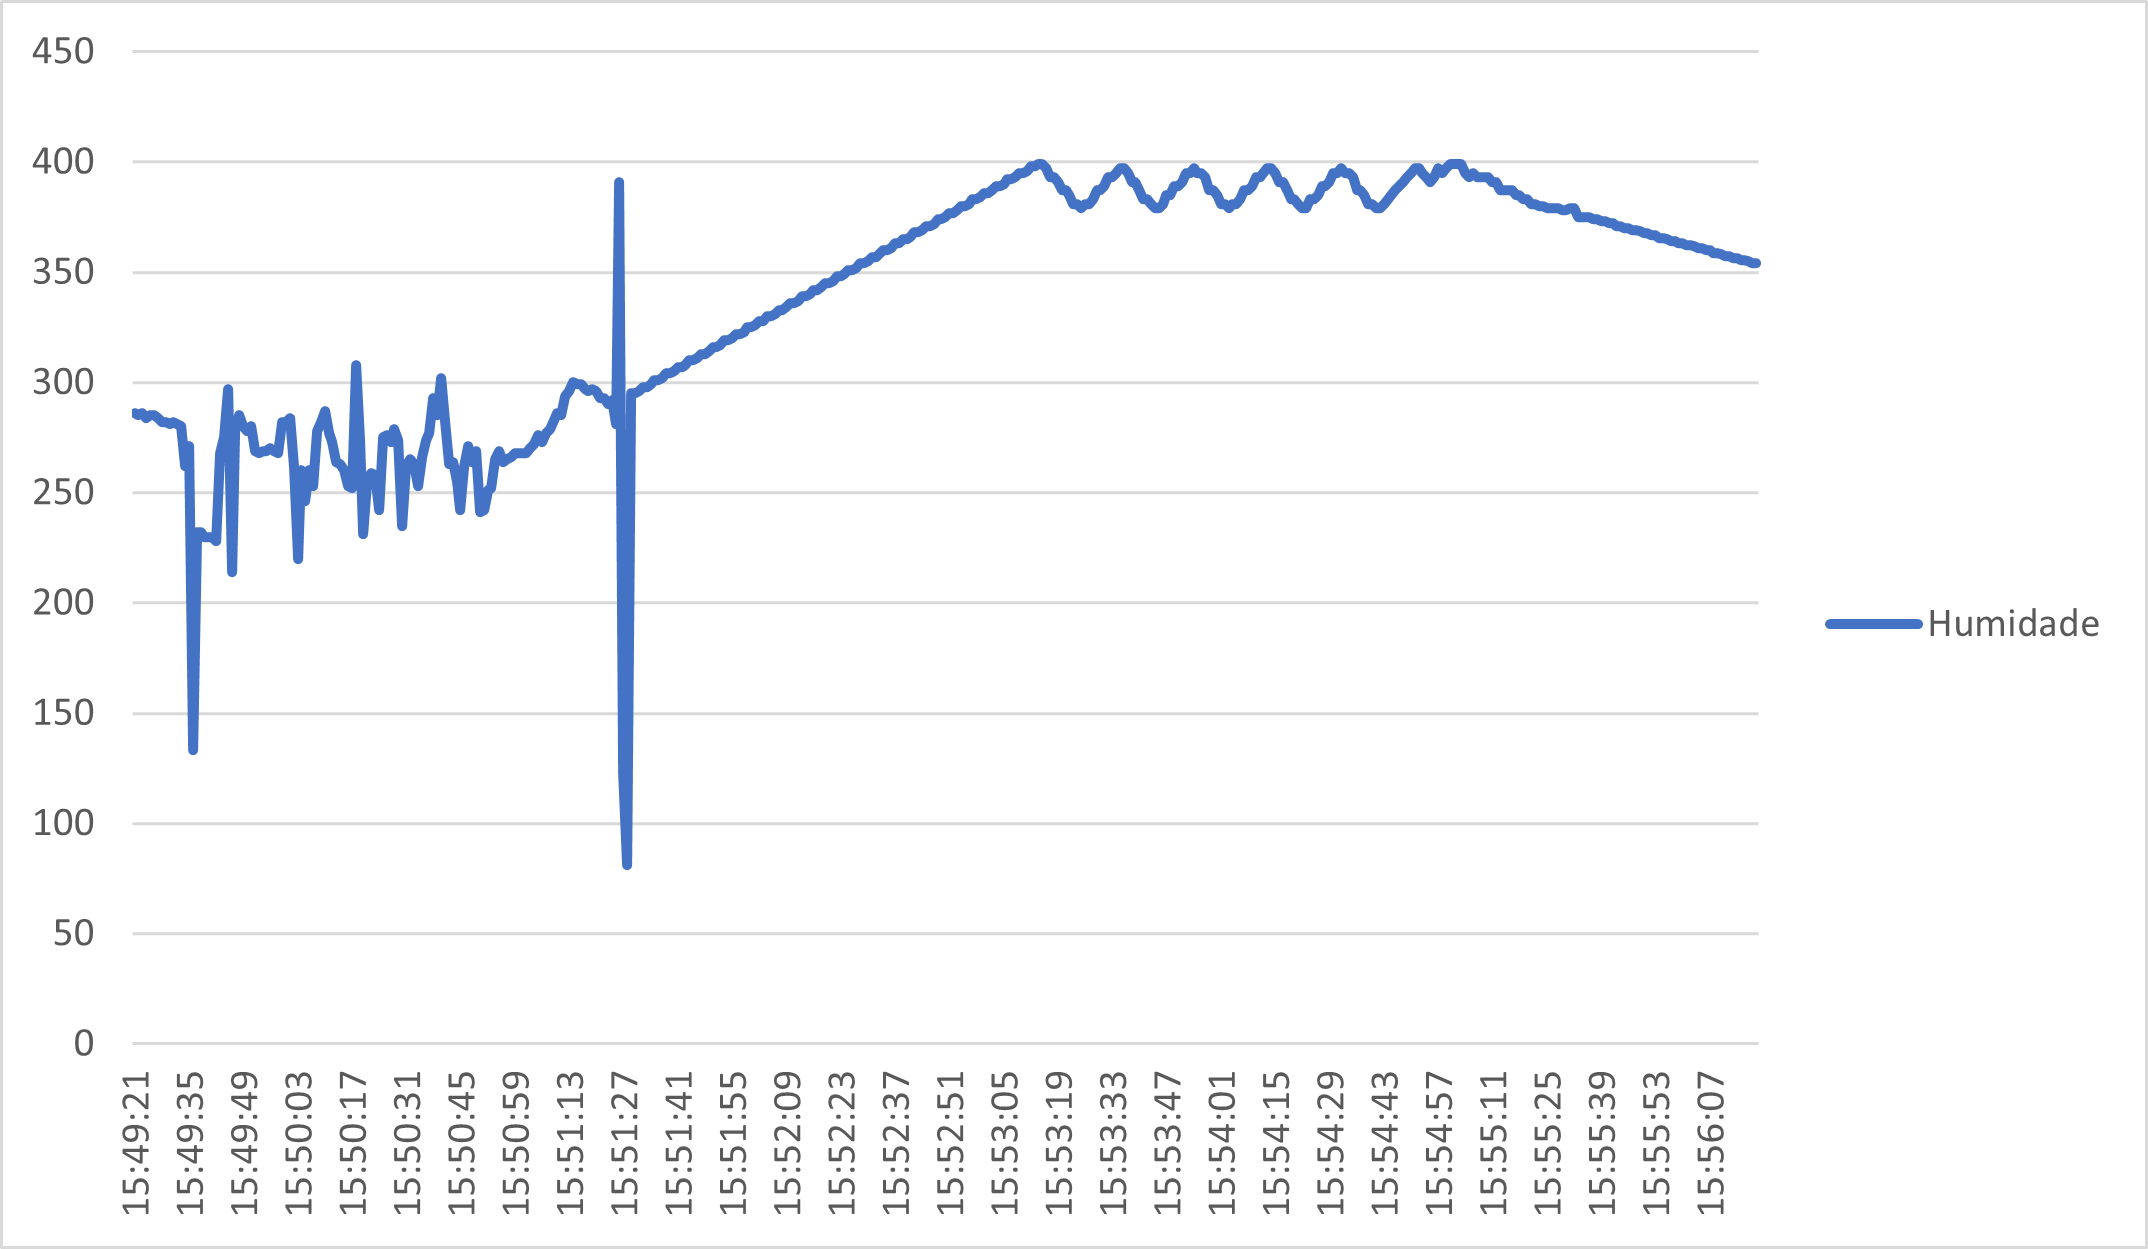
\includegraphics[scale=0.5]{humidity-test-graph.png}
    \caption{Gráfico dos resultados do teste realizado}
    \label{fig:graphic}
\end{figure}

Os resultados obtidos revelaram ser muito abaixo dos valores esperados. Sendo que nos testes preliminares 
foi possível obter valores muito mais elevados, tal que foi possível testar o limite máximo do sensor. Seria 
expectável que os resultados obtidos através dos testes estivessem mais próximo dos valores verificados 
durante as simulações. Um valor expectável para o solo húmido seria um valor entre os 600 e os 700, sendo 
um valor superior a 750 seria considerado como solo demasiado húmido.

Dos testes realizados, verificou-se em dois casos diferentes que para um tipo de solo o valor máximo obtido foi 
de cerca de 300 e para o caso representado pelo gráfico da figura \ref{fig:graphic} o valor máximmo 
obtido foi de 400.
Isto deve-se ao facto de nos dois casos, apesar de se estar a realizar testes com o mesmo tipo de plantas, 
cada uma das plantas estava plantada em tipos de solo diferentes. A primeira estava plantada num vaso de 
pequenas dimensões em que o solo é um composto de turfa loira de Sphagnum \cite{jardinssintra}, 
como mostra a figura \ref{fig:testconditions}, enquanto que o teste descrito neste artigo, 
a planta encontra-se plantada em terra. 

\begin{figure}[h]
    \centering
    \includegraphics[width=0.3\textwidth]{rosas-solo-composto.jpg}
    \caption{Plantas no solo de composto Sphagnum}
    \label{fig:testconditions}
\end{figure}

Como mencionado no artigo de Abbas et al. \cite{abbas2014smart}, diferentes solos têm diferentes características 
sendo uma delas a capacidade de retenção de água. Isto poderá ser um dos factores, não considerados pelos 
discentes, que terá tido influência nos resultados obtidos.

\section{Conclusão e Trabalho Futuro}

Um dos maiores problemas que vamos enfrentar num futuro próximo é a escassez de água potável,
e sendo a água um bem essencial para a sobrevivência humana, existe uma preocupação 
em criar sistemas que possibilitem uma melhor gestão da água. Por isto mesmo 
é que proposmos este sistema de rega de água inteligente. Apesar de não ser um 
sistema muito robusto e que pela sua natureza funciona melhor em pequena escala, este 
poderia ser uma ponte para a criação de um sistema mais robusto que funciona-se bem 
tanto áreas pequenas como jardins ou estufas, como também em áreas maiores como campos agrículas.

Para trabalho futuro poderia ser integrado um Raspberry Pi neste sistema para uma melhor 
gestão de informação. Um dos pontos fracos que o sistema proposto tem é não 
ter em conta a previsão do tempo o que pode tornar este sistema menos eficiente. 
Esta previsão de tempo poderia ser integrada no sistema através de um API que 
envia os dados de previsão em tempo real e juntamente com os dados do sensor de 
humidade o sistema tomaria a decisão se regava as plantas ou não.

Este sistema, tal como os sistemas convencionais, também poderia funcionar em horários definidos, 
visto que os sistema proposto apenas utiliza a humidade do solo, numa estação de maior calor, a humidade do solo 
irá se reduzir a um ritmo mais acelerado do que numa estação onde as temperaturas são mais baixas. Desta forma, 
seria possível poupar ainda mais água, bem como energia elétrica, visto que o sistema apenas estaria ligado apenas 
nas horas indicadas. Sendo que o sensor de humidade do solo, irá se degradar com o tempo, também ajudaria a 
longevidade do sistema.

Não foi possível implementar uma interface gráfica para monitorização do sistema, como era pretendido. 
O Arduino MKR 1010 wifi foi o microcontrolador escolhido pelo facto de ter capacidade de ligação à Internet. 
Desta forma, os dados recolhidos poderiam ser enviados para a Arduino Cloud onde o utilizador do sistema poderia, 
então, monitorizar o sistema através do seu smartphone. No entanto, como já referido, não possível 
implementar tal interface.

Seria necessário, também a realização de mais testes, visto que os valores obtidos estiveram abaixo do 
esperado. Como mencionado no artigo de Abbas et al. \cite{abbas2014smart}, 
sabe-se que diferentes solos têm características diferentes e que devido a estas diferenças, existem outros 
fatores a considerar para um sistema de rega inteligente, tais como a capacidade de retenção de água do solo, 
a estação do ano, mas também outros fatores como o tipo de plantas para o qual o sistema será utilizado.

\subsection{Problemas Encontrados}

Durante a realização do projeto descrito neste artigo, surgiram vários problemas, tanto com o hardware 
assim como com o software.

A grande maioria dos problemas encontrados com o hardware estavam relacionados com o mau funcionamento dos 
dispositivos eletrónicos e com más ligações entre os componentes. A solução para estes problemas foi a 
substituição dos mesmo componentes, especialmente alguns cabos.

Os problemas de software estavam relacionados com o editor de texto e o programa do Arduino. Alguns dos problemas 
foram resolvidos com a instalação de dependências e bibliotecas para a placa Arduino MKR 1010 wifi. 
O problema que atrasou mais o desenvolvimento do projeto é um erro do software Arduino nos quais não era possível 
detetar a placa quando estava ligada a uma das entradas USB do computador. Para se encontrar a resolução 
consultou-se os vários fóruns, em especial, o fórum da comunidade Arduino. Uma das possíveis soluções era a 
reinstalação do software bem como todas as dependências e bibliotecas necessárias. Outra solução é colocar a 
placa Arduino em modo bootloader. \cite{arduinoport}

\bibliographystyle{IEEEtran}
\bibliography{references}

\end{document}
